\chapter{Mathematical Background}

The purpose of this chapter is to remind the reader basic notions regarding algebra and statistics, but also to analyze in detail concepts and algorithms concerning lattices, especially integer lattices. 

\section {Algebra}
The notions of group, cyclic group, ring and polynomial are considered to be previously known by the average reader. More information about the mentioned structures can be found in \cite{HPS08}, chapter 2. For a mathematical perspective over groups and polynomial rings properties, and also for a deep incursion in field extension theory, the reader can explore \cite{BB15}.

\begin{enumerate}
	\item \textbf{Ideals and Quotient Rings.} 
	
	\textbf{Definition 5.} \textit{Let $(R, +, \cdot)$ be a commutative finite ring. An \textbf{ideal} of $R$ is a nonempty set $\ci \subseteq R$ that is closed under addition and $ax=xa \in \ci, \forall x \in \ci, \forall a \in R.$} \\
	
	Let $(R, +, \cdot)$ be a finite ring and $\ci$ be an ideal of $R$. Also, let $"\sim"$ be an equivalence relationship on $R$, defined by $x \sim y \iff \exists a\in \ci $ such that $x = y + a$. The equivalence class of an element $x \in R$ is usually noted with $\hat{x}$, and it represents the set $\{y \in R : y \sim x\}$. The equivalence classes generate a partition of the set $R$, named \textit{quotient set}, and denoted by $R/\ci$. It is known that $(R/\ci, +, \cdot)$ is also a ring, and it is called the \textbf{quotient ring} $R/\ci$.
	
	\textbf{Remark 3.} \textit{An example of a quotient ring is the well-known ring $\bZ_p = \bZ/p\bZ.$}
	
	\item \textbf{Cyclotomic polynomials.}
	
	\textbf{Definition 6 \cite{BB15}.} \textit{Let $n \geq 1$ be an integer and $P_n $ be the set of all the $n^{th}$ primitive roots of unity. Then, the \textbf{$n^{th}$ cyclotomic polynomial} is $\Phi_n = \displaystyle{\prod_{\xi \in P_n}}(X-\xi)$}.
	
	\textbf{Remark 4.} Using the fact that $\Phi_{p^k}(X) = \Phi_p(X^{p^{k-1}})$, for any positive integers $k, p$, with $p-$prime, it can be proved that $\Phi_{2^k}(X) = X^{2^{k-1}} + 1,$ for any integer $k \geq 1$.
	
	\item \textbf{Vector spaces}.
	
	Throughout the paper, vectors and matrices are thickened, e.g. $\textbf{v}$. Also, every vector space is considered to be contained in $R^m$, with $m \geq 1$, integer.\\
	
	\textbf{Definition 7 \cite{HPS08}.} \textit{Let $m$ be a positive integer. A \textbf{vector space} $V$ is a subset of $\bR^m$, such that for every $\alpha_1, \alpha_2 \in \bR$ and every} $\textbf{v}_1, \textbf{v}_2 \in V$, it holds: $\alpha_1 \vv_1 + \alpha_2 \vv_2\in V$.
	
	The lecturer is expected to master the concepts of \textit{linear combination, linear independence, basis, vector orthogonality, basis orthogonality}. For a quick review over the mentioned concepts, visit \cite{HPS08}.\\
	
	The only algorithm regarding vector spaces to be presented in the current paper is the  \textbf{Gram-Schmidt Algorithm}. It receives as input a basis $\{\vv_1, .., \vv_n\}$ of the vector space $V$ and outputs $\{\vv_1^*,..,\vv_n^*\}$ - an orthonormal basis of $V$. The algorithm is presented below:

\begin{tcolorbox}[colframe=black,colback=white,arc=0pt,outer arc=0pt]
	\begin{algorithmic}[1]
		\State Set $\vv_1^* = \vv_1$
		\For{$i \la 2$ \textbf{to} $n$}
		\State Compute $\mu_{ij} = \vv_i \cdot \vv_j^*$ $/$ $ ||\vv_j^*||$,  for $1 \leq j < i$
		\State Set $\vv_i^* = \vv_i - \displaystyle{\sum_{j = 1}^{i-1}} \mu_{ij} \vv_j^* $
		\EndFor
	\end{algorithmic}
\end{tcolorbox}

	Intuitively, $\mu_{ij}$ represents the length of the projection of $\vv_i$ over $\vv_j^*$. Therefore, the substraction $\vv_i - \mu_{ij} \vv_j^*$ generate the projection of $\vv_i$ over the orthogonal complement of $\vv_j^*$, which leads to the desired output. 
\end{enumerate}	

\section{Lattices}

\subsection{General Influence}

Lattices have been studied by mathematicians such as Gauss, Lagrange or Minkowski since 18$^{th}$ century, and have been used to prove theorems in number theory and the field extensions. Even though lattices confirmed their significance in mathematics, they were not used in computer science until the 1980s, when Lenstra, Lenstra and Lov\`{a}sz proposed the basis-reduction algorithm \textbf{LLL}. It represented a major breakthrough in cryptography, and was used to break several cryptosystems, such as RSA (in a low exponent setting) and NTRU. \\

Since the proposal of \textbf{LLL} algorithm, lattices became appealing to the world of cryptography. Thus, since then they have been used in the construction of cryptographic schemes, such as Attribute Based Encryption \cite{Boy13}, Fully homomorphic encryption \cite{Gen09} and Graded Encoding Systems \cite{GGH13}.

\subsection{Basic Concepts}

\textbf{Definition 8 (\cite{HPS08}).} \textit{Let $n, m$ be two positive integers and let} $B = \{\vv_1, .., \vv_n\} \subset \bR^m$ \textit{ be a set of linearly independent vectors. The \textbf{lattice} generated by $B$ is the set:}
\begin{center}
	$L$   $  \stackrel{\mathclap{\normalfont\mbox{not.}}}{=} \mathcal{L}(B) = \{a_1\vv_1 + a_2 \vv_2 +... + a_n\vv_n : a_1, a_2, ..,a_n \in \bZ\}$.
\end{center}

\textit{Also, a lattice that contains only vectors with integer coordinates is called an \textbf{integer lattice}}.

From a visual point of view, the elements of a lattice are structured as a net, with massive holes between the nodes, as it can be noticed in Figure 1.
\newpage

\textbf{Definition 9 (\cite{HPS08}).} \textit{Let $L$ be a $n$-dimensional lattice and} $B = \{\vv_1,...,\vv_n\}$ \textit{be a basis for the lattice $L$. The \textbf{fundamental domain} for $L$ that is associated with $B$ is:}
\begin{center}
	$\mathcal{F}(\vv_1,...,\vv_n) = \{t_1\vv_1 + ...+ t_n\vv_n : t_i \in [0, 1], \forall i \in \{1,..., n\}\}$.
\end{center}

\begin{center}
	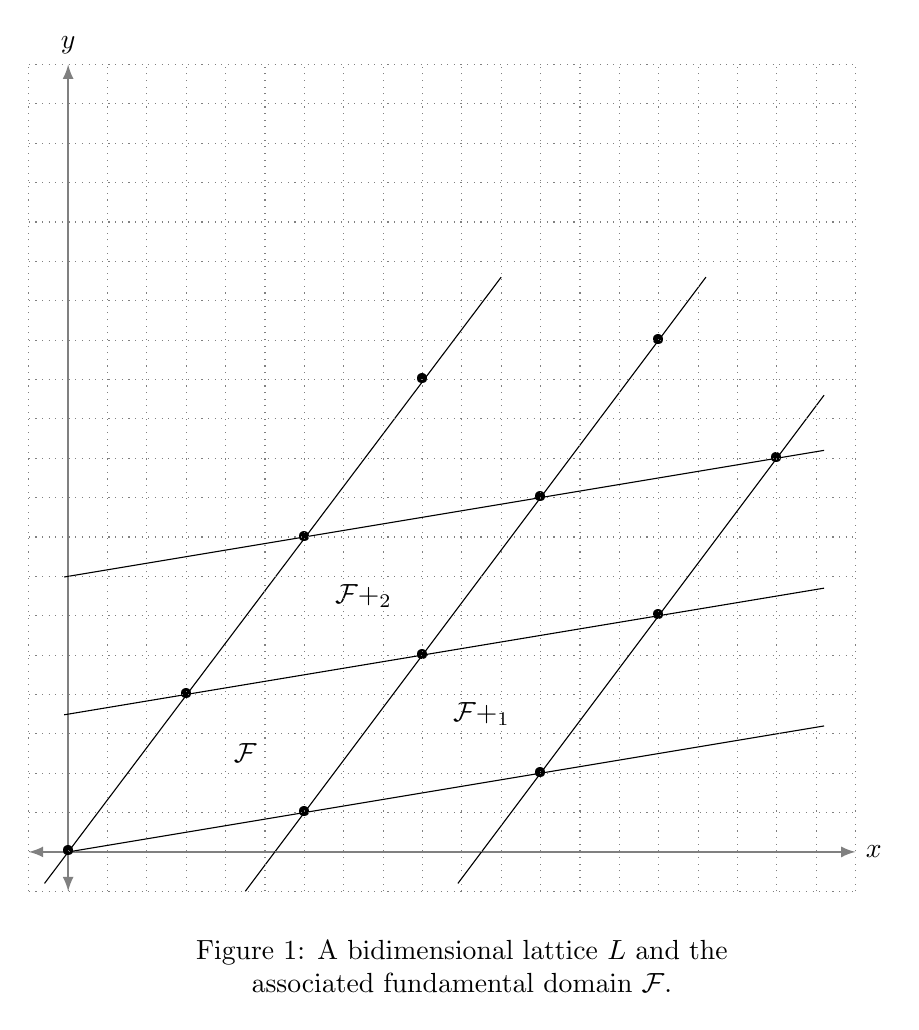
\begin{tikzpicture}[scale = 0.5]
\draw[latex-latex, thick, draw=gray] (-1,0)--(20,0) node [right] {$x$}; 
\draw[latex-latex,thick, draw=gray] (0,-1)--(0,20) node [above] {$y$};

\foreach \Point in {(0, 0), (3, 4), (6,1), (9, 5), (6, 8), (9, 12), (12, 9), (15, 13), (12,2), (15, 6), (18, 10)}{
	\node at \Point {\textbullet};
}

\draw[black] (-0.6, -0.8) -- (11, 14.6);
\draw[black] (4.5, -1) -- (16.2, 14.6);
\draw[black] (9.9, -0.8) -- (19.2, 11.6);

\draw[black] (-0.1, -0.0166) -- (19.2, 3.2);
\draw[black] (-0.1, 3.483333) -- (19.2, 6.7);
\draw[black] (-0.1, 6.983333) -- (19.2, 10.2);


\node [black] at (4.5,2.5) {$\mathcal{F}$};
\node [black] at (10.5,3.5) {$\mathcal{F}+ \vv_1$};
\node [black] at (7.5,6.5) {$\mathcal{F}+ \vv_2$};
\draw [dotted, gray] (-1,-1) grid (20,20);

\node [below=1cm, align=flush center,text width=8cm] at (10, 0)
{
	Figure 1: A bidimensional lattice $L$ and the associated fundamental domain $\mathcal{F}$.
};
\end{tikzpicture}
\end{center}

\textbf{Proposition 2.} \textit{Let $n$ be a positive integer and $L \subset \bR^n$ be a lattice of dimension $n$. Then, for every basis $B$ of $L$, the volume of the fundamental domain associated with it is the same.}\\

\textbf{Definition 10.} \textit{Let $n$ be a positive integer and let $L \subset \bR^n$ be a lattice of dimension $n$. The \textbf{determinant} of $L$ is the volume of any fundamental domain for $L$, and it is denoted by det($L$).}

\subsection{Hard problems}

In order to be able to use lattices in the design of cryptographic schemes, it is required that hard problems related to them to be known. Some of the most important hard problems related to lattices are presented below \cite{HPS08}:

\begin{itemize}
	\item  \textbf{Shortest Vector Problem (SVP).} Let $n$ be a positive integer and $L$ be a lattice of dimension $n$. The problem to find a vector $\vv = \displaystyle{\argmin_{ \textbf{w} \in L \backslash \{\textbf{0}\}}} ||\textbf{w}||$ is referred to as \textbf{SVP}.\\
	
	\item \textbf{Closest Vector Problem (CVP).} Let $n$ be a positive integer and $L$ be a lattice of dimension $n$. Also, let $\textbf{w}$ be a vector in $\bR^n \backslash L$. The problem to find a vector $\vv\in L$ that satisfies $||\textbf{w} - \vv|| = \displaystyle{\min_{ \textbf{u} \in L}} ||\textbf{w} - \textbf{u} || $ is called \textbf{CVP}.\\
	
	\item \textbf{Approximate Shortest Vector Problem (apprSVP).} Let $\psi : \bN \ra \bR$ be a function of one parameter and let $\lambda_1(L) \in L$ be one of the shortest vectors in $L$ (i.e. a solution to \textbf{SVP}). The problem to find a vector $\vv \in L \backslash \{\textbf{0}\}$ such that $||\vv|| \leq \psi(n) \cdot || \lambda_1(L) ||$ is called \textbf{apprSVP}.\\

	\item \textbf{Approximate Closest Vector Problem (apprCVP).} Let $\psi : \bN \ra \bR$ be a function of one parameter, let $\textbf{u} \in \bR^n \backslash L$ be a non-lattice vector and let $\textbf{w}$ be a solution to \textbf{CVP} associated with $\textbf{u}$. The problem to find a vector $\vv \in L$ such that $||\vv - \textbf{u} || \leq \psi(n) \cdot ||\textbf{w} - \textbf{u}||$ is called \textbf{apprCVP}.
\end{itemize}

\textbf{Remark 5. } \textit{\textbf{apprSVP} is known to be hard to solve, even for polynomial approximation functions $\psi$. Also, it is resistant to quantum computing attacks, as opposed to integer factorization problem, which becomes easy in a quantum computing environment, using Schor's algorithm.}

\subsection{Results concerning short vectors}

In order to verify how accurate is the returned solution of an approximation algorithm, it is needed to have an estimate of the desired result. Therefore, an approximative value of the shortest vector length in a lattice is necessary for testing the result of an algorithm solving \textbf{apprSVP}. \\

The current subsection only states the most important results regarding shortest vector length in a lattice. The lecturer who is interested in the proofs of the following results may find them in \cite{HPS08}.\\

\textbf{Definition 11.} \textit{Let $n$ be a positive integer and $L$ be a lattice of dimension $n$. Also, let} $B = \{\vv_1,...,\vv_n\}$ \textit{be a basis of $L$. The \textbf{Hadamard ratio} is defined by:}
\begin{center}
	$\mathcal{H}(B) = \Big(\frac{\text{det}(L)}{||\vv_1|| \cdot ||\vv_2|| \cdot ... \cdot ||\vv_n||} \Big)^{1/n}$.
\end{center}
\textit{The Hadamard ratio is a real number in the interval (0, 1] and it represents a measure of the orthogonality of the basis $B$, with the understanding that the closer the Hadamard ratio is to 1, the more orthogonal are the vectors in $B$.}\\

\textbf{Theorem 1 (Minkowski's Theorem \cite{HPS08}).} \textit{Let $n$ be a positive integer and $L\subset \bR^n$ be a lattice of dimension $n$. If $S \subset \bR^n$ is a symmetric convex set with the property that} $Vol(S) > 2^n \text{det}(L),$ \textit{then $S$ contains a nonzero lattice vector. If $S$ is also a closed set, then it is sufficient to verify that }$Vol(S) \geq 2^n \text{det}(L)$. \\

\textbf{Theorem 2 (Hermite's Theorem \cite{HPS08}).} \textit{Let $n$ be a positive integer. Then, for every lattice $L$ of dimension $n$, there exists a vector} $\vv \in L \backslash\{\textbf{0}\}$ \textit{such that}  $||\vv|| \leq \sqrt{n} \cdot \text{det} (L) ^{1/n}$.\\

\textbf{Remark 6.} \textit{The Hermite's Theorem is a consequence of Minkowski's Theorem, where the set $S$ is considered to be a hypercube in $\bR^n$ centered at \textbf{0}. Considering $S$ to be a hypersphere instead of a hypercube, centered at \textbf{0}, the upper bound in Hermite's theorem is lowered by a factor of $\sqrt{\frac{2}{\pi e}}$}.\\

\textbf{Proposition 3 (\cite{HPS08}).} \textit{Let $n$ be a positive integer and $L\subset \bR^n$ be a lattice of dimension $n$. The \textbf{Gaussian heuristic} affirms that the length of the shortest nonzero vector in $L$ is expected to be} $\sigma(L) = \sqrt{\frac{n}{2\pi e}}\big(\text{det}(L)\big)^{1/n}$.

The vigilant reader may note that the \textit{gaussian expected shortest length} is two times smaller than the upper bound presented in \textit{Remark 6}. \\

\subsection{Attempts to solve hard lattice problems}



